\documentclass[11pt]{article}

\usepackage[margin=1.15in]{geometry}
\usepackage[T1]{fontenc}
\usepackage{lmodern}
\usepackage{microtype}
\usepackage{amsmath,amssymb,amsthm,mathtools}
\usepackage{enumitem}
\usepackage{booktabs}
\usepackage{tikz}
\usetikzlibrary{positioning,decorations.pathreplacing}
\usepackage{xcolor}
\usepackage{url}
\usepackage{aliascnt}
\usepackage[colorlinks=true,linkcolor=blue!50!black,citecolor=green!35!black,urlcolor=blue!50!black]{hyperref}
\usepackage[capitalize,nameinlink]{cleveref}

% ---------------------------------------------------------------------------
% Lean declarations are typeset in typewriter type and may break at dots.
\DeclareUrlCommand\lean{\urlstyle{tt}}
\newcommand{\leanref}[1]{{\unskip\nobreak\hfil\penalty50\hskip1em\null\nobreak\hfil
  {\normalfont\small\lean{#1}}\parfillskip=0pt\finalhyphendemerits=0\par}}

% Each environment gets its own counter, aliased to the shared one, so that cleveref
% names references by their environment.
\newcommand{\sharedtheorem}[2]{%
  \newaliascnt{#1}{theorem}\newtheorem{#1}[#1]{#2}\aliascntresetthe{#1}%
  \crefname{#1}{#2}{#2s}}
\theoremstyle{plain}
\newtheorem{theorem}{Theorem}[section]
\sharedtheorem{lemma}{Lemma}
\sharedtheorem{proposition}{Proposition}
\sharedtheorem{corollary}{Corollary}
\theoremstyle{definition}
\sharedtheorem{definition}{Definition}
\sharedtheorem{hypothesis}{Hypothesis}
\theoremstyle{remark}
\sharedtheorem{remark}{Remark}
\sharedtheorem{example}{Example}
\crefname{hypothesis}{Hypothesis}{Hypotheses}

\newcommand{\N}{\mathbb{N}}
\newcommand{\R}{\mathbb{R}}
\newcommand{\Acc}{\mathrm{Acc}}
\newcommand{\cut}{\delta}
\newcommand{\rect}{\mathcal{R}}
\newcommand{\LB}{\mathrm{LB}}
\newcommand{\restr}[2]{#1|_{#2}}
\newcommand{\card}[1]{\lvert #1\rvert}
\newcommand{\rd}{\mathrm{read}}
\newcommand{\site}{\mathrm{site}}
\DeclareMathOperator{\cw}{cw}
\DeclareMathOperator{\pw}{pw}

\title{The Frontier Method\\[0.4em]
\large Circuit lower bounds from graph layouts, with a formal proof}
\author{Samuel Schlesinger}
\date{Draft of October 2026}

\begin{document}
\maketitle

\begin{abstract}
Order the gates of a circuit along a line and cut the line anywhere. Whatever the inputs on
one side tell the computation on the other side must cross the cut, carried by the wires that
span it. We make this picture exact and quantitative. A circuit of size $s$ whose gates have
fan-in at most $r$ compiles into a constraint network of maximum degree $r+1$ whose cycle rank
is at most $(r-1)s - n + o(n)$. A layout of the network in which every frontier carries at most
$w$ values yields a read-once protocol for the accepted inputs whose messages have $w$ symbols.
If the accepted set is dense and $K$-rectangle-free with $\log K = o(n)$, every such protocol
needs $w \ge n - o(n)$. Consequently, any layout theorem of the form
$\cw(G) \le (A + o(1))\,\beta_1(G) + o(\card{V(G)})$ for graphs of maximum degree $r+1$
forces $(r-1)s \ge (L - o(1))\,n$ with $L = 1 + 1/A$, over every basis of fan-in $r$ on every
finite alphabet.
For fan-in two we prove the layout bound with
$A = \frac{3}{\pi}\arccos\frac{1+2\sqrt2}{4} \approx 0.2807$, by ordering the vertices of a
cubic graph by the median of correlated Gaussian edge scores; this gives a lower bound of
$(L - \varepsilon)n$ with $L = 1 + 1/A \approx 4.5625$, and in particular $(4 - \varepsilon)n$.

The proof factors into five independent pieces: a combinatorial property of the hard set, an
abstract counting lemma for read-once protocols, a separator property of constraint networks,
a compiler from circuits to networks, and a layout theorem from graph theory. All five are
formalized in Lean~4 on CSLib and Mathlib.
\end{abstract}

\tableofcontents

% ===========================================================================
\section{Introduction}
\label{sec:intro}

\subsection{The theorem}

A \emph{circuit} over a finite alphabet $U$ is a straight-line program: each gate applies an
operation $U^{a} \to U$ of some arity $a$ to inputs and earlier gates. Its \emph{size} is the
number of gates; its \emph{fan-in} is the largest arity. A circuit with a designated output
\emph{decides} a set $S \subseteq U^n$ if, for some set $\Acc \subseteq U$ of accepting values,
an input lies in $S$ exactly when the output lies in $\Acc$. No assumption is made about which
operations are available: the basis may be any set of operations, including all of them.

A set $S \subseteq U^n$ is \emph{$K$-rectangle-free} if, however the $n$ coordinates are split
into two groups, every combinatorial rectangle contained in $S$ has a side with fewer than $K$
elements (\cref{def:rectangle-free}). The theorem needs one fact from graph theory, a
\emph{layout bound}: graphs of maximum degree $d$ can be laid out on a line so that every cut
between an initial segment and the rest is crossed by at most $A\,\beta_1 + o(\card V)$ edges,
where $\beta_1 = \card E - \card V + 1$ is the cycle rank (\cref{hyp:layout}).

\begin{theorem}[Main theorem]
\label{thm:main}
Let $r \ge 2$ and $A > 0$, and assume the layout bound $\LB_{r+1}(A)$. Let $U$ be an alphabet
with $q \ge 2$ symbols, and for every $n$ let $S_n \subseteq U^n$ be $K_n$-rectangle-free with
\[
  \log K_n = o(n) \qquad\text{and}\qquad \log \card{S_n} \ge n \log q - o(n).
\]
Then for every $\varepsilon > 0$ and all sufficiently large $n$, every circuit of size $s$ and
fan-in at most $r$ that decides $S_n$, over any basis on $U$, satisfies
\[
  (r - 1)\, s \;>\; \Bigl(1 + \frac1A - \varepsilon\Bigr)\, n .
\]
\leanref{Frontier.lowerBound}
\end{theorem}

We call $L = 1 + 1/A$ the \emph{circuit coefficient} of the layout coefficient $A$. For fan-in
two the graphs are subcubic, and the bound is on the size itself.

\begin{corollary}[Fan-in two]
\label{cor:fanin-two}
Under $\LB_3(A)$, every circuit of fan-in at most two deciding $S_n$ has more than
$(L - \varepsilon)\,n$ gates for all large $n$, where $L = 1 + 1/A$.
\leanref{Frontier.lowerBound_fanInTwo}
The layout coefficients are those of \cref{sec:layouts}; both are proved:
\begin{center}
\begin{tabular}{lcc}
\toprule
layout theorem & $A$ & $L = 1 + 1/A$ \\
\midrule
Gaussian edge scores & $\approx 0.2807$ & $\approx 4.5625$ \\
weakening ($2p \le 9/32$) & $1/3$ & $4$ \\
\bottomrule
\end{tabular}
\end{center}
The Gaussian coefficient is $A = \frac{3}{\pi}\arccos\frac{1+2\sqrt2}{4}$, so that
$L = 1 + \pi \big/ \bigl(3 \arccos\frac{1+2\sqrt2}{4}\bigr)$
(\lean{Frontier.lowerBound_gaussian}, \lean{Frontier.lowerBound_four}).
\end{corollary}

The hypotheses on $S_n$ are satisfiable: a uniformly random subset of $\{0,1\}^n$ is
$(n+2)$-rectangle-free with high probability (\cref{prop:random}). Of course a random set has
no small circuit at all; the content of \cref{thm:main} is for explicit sets. Explicit dense
rectangle-free families in $\mathsf{P}$, with $\log K_n = o(n)$, can be built from extractors
for the sum of two sources~\cite{ChattopadhyayLiao2021,Li2023}.
For the full binary basis $B_2$ the strongest previously published lower bound for an explicit
function is $(3.1 - o(1))\,n$, due to Li and Yang~\cite{LiYang2022}, improving the
$(3 + 1/86)\,n$ of Find, Golovnev, Hirsch, and Kulikov~\cite{FGHK2016}.

\subsection{The idea}

Three sentences carry the proof.

\paragraph{Gates create local constraints.}
Forget that a circuit computes. Put a value on every wire and ask only that each gate's output
value equal its operation applied to its input values. For a fixed input, the run of the
circuit is the unique assignment satisfying all of these local equations. The equations are
\emph{relations}: a gate $z = g(x,y)$ is the set of triples $(x,y,z)$ with $z = g(x,y)$, and
nothing ever needs to invert $g$.

\paragraph{Fan-out creates topology.}
To make every constraint see a bounded number of values, a wire read by many gates is routed
through a chain of copy vertices. The resulting constraint graph has maximum degree $r+1$, and
its cycle rank is about $(r-1)s - n$. A formula, in which every wire is read once, compiles to a
tree. Every gate beyond those of a formula adds an independent cycle.

\paragraph{A frontier value is exactly the message sent by the past to the future.}
Lay the constraint graph out on a line, in any order whatsoever, unrelated to the order of
evaluation. After the first $t$ vertices, the edges between the processed and the unprocessed
vertices form the \emph{frontier}. Once the values on the frontier are fixed, the two sides of
the constraint system are independent (\cref{lem:separator}). So the frontier values are a
message from the inputs read so far to the inputs not yet read, and the sequence of frontiers
is a read-once protocol for the accepted set. A rectangle-free set needs messages of about $n$
symbols at some step (\cref{lem:counting}). A layout bound produces frontiers of about
$A\,\beta_1 \approx A((r-1)s - n)$ edges. Comparing the two gives $n \lesssim A((r-1)s - n)$.

\subsection{How the proof is factored}

\begin{center}
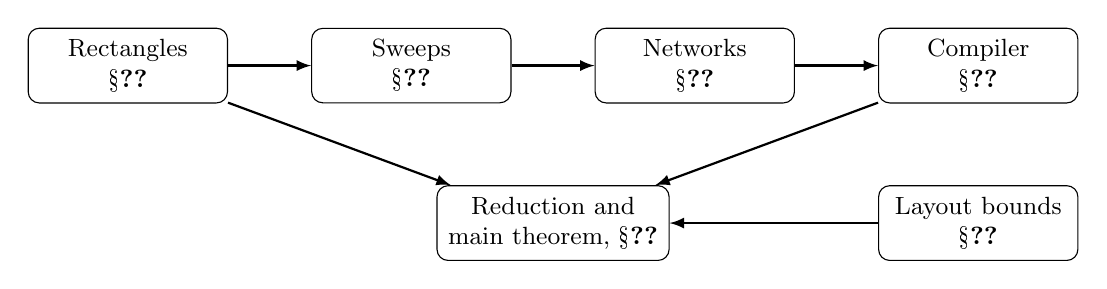
\begin{tikzpicture}[
  box/.style={draw, rounded corners, align=center, font=\small, minimum height=2.6em,
    minimum width=7.2em, inner sep=4pt},
  arr/.style={-latex, thick}]
\node[box] (rect) at (0, 0) {Rectangles\\ \S\ref{sec:rectangles}};
\node[box] (sweep) at (3.6, 0) {Sweeps\\ \S\ref{sec:sweeps}};
\node[box] (net) at (7.2, 0) {Networks\\ \S\ref{sec:networks}};
\node[box] (comp) at (10.8, 0) {Compiler\\ \S\ref{sec:compiler}};
\node[box] (red) at (5.4, -2) {Reduction and\\ main theorem, \S\ref{sec:lowerbound}};
\node[box] (lay) at (10.8, -2) {Layout bounds\\ \S\ref{sec:layouts}};
\draw[arr] (rect) -- (sweep);
\draw[arr] (sweep) -- (net);
\draw[arr] (net) -- (comp);
\draw[arr] (rect) -- (red);
\draw[arr] (comp) -- (red);
\draw[arr] (lay) -- (red);
\end{tikzpicture}
\end{center}

\begin{description}[leftmargin=1.5em, itemsep=0.2em]
\item[Rectangles (\cref{sec:rectangles}).] The only property of the hard set, and the support
  lemma: a dense rectangle-free set depends on all but $\log_q K$ coordinates.
\item[Sweeps (\cref{sec:sweeps}).] An abstract read-once protocol and the \emph{frontier
  counting lemma}: a $K$-rectangle-free set has at most $(K-1)^2$ elements per transition. No
  graphs or circuits appear.
\item[Networks (\cref{sec:networks}).] Constraint networks, the separator lemma, and the sweep
  of a network along a layout, with $\card U^{w + O(1)}$ transitions per step.
\item[Compiler (\cref{sec:compiler}).] Circuits of fan-in $r$, over any basis, become exact
  constraint networks of maximum degree $r+1$ and cycle rank at most $(r-1)s + 1 - \card{\rd}$.
\item[Reduction and main theorem (\cref{sec:lowerbound}).] A small circuit yields a graph of
  small cycle rank all of whose layouts are wide; a layout bound finishes the proof.
\item[Layout bounds (\cref{sec:layouts}).] The graph theory: compressing to cubic graphs,
  median layouts, and Gaussian edge scores give the coefficient $A \approx 0.2807$.
\end{description}

Each piece has a one-line interface, and each could be replaced independently. A better hard
set improves nothing (the coefficient depends only on $A$), a better layout theorem improves
the coefficient directly, and a different notion of message capacity, such as rank in place of
counting, transfers the whole argument to arithmetic circuits (\cref{sec:extensions}).

\subsection{The formalization}

Everything in this paper except \cref{prop:random} is formalized in Lean~4~\cite{Lean4}
(toolchain \texttt{v4.35.0-rc3}), using Mathlib~\cite{Mathlib} (commit \texttt{9a6fbe0}) and
CSLib~\cite{CSLib} (commit \texttt{89dc6fb}), in about 5,500 lines including documentation. The circuit model is CSLib's: signatures, interpretations,
straight-line programs, and circuits. Every result below is tagged with the Lean declaration
that proves it. The main theorem and every result it uses depend only on Lean's standard
axioms (\texttt{propext}, \texttt{Classical.choice}, \texttt{Quot.sound}); there is no
\texttt{sorry}. The layout bound $\LB_d(A)$ is a Lean definition (\lean{Frontier.LayoutBound}):
the main theorem takes it as a hypothesis, so that any layout theorem can be plugged in, and
\cref{thm:layout} proves it for $d = 3$. \Cref{sec:design} records the design decisions
behind the formal statements, and \cref{app:index} is an index from the paper to the code.

% ===========================================================================
\section{Rectangles}
\label{sec:rectangles}

Throughout, $\iota$ is a finite set of \emph{coordinates} and $U$ a finite \emph{alphabet}
with $q = \card U$ symbols. An \emph{input} is a function $x \colon \iota \to U$. For
$X \subseteq \iota$ we write $\restr{x}{X}$ for the restriction of $x$ to $X$, its
\emph{part} on $X$, and $X^c$ for $\iota \setminus X$. An input is determined by its two parts
$\restr{x}{X}$ and $\restr{x}{X^c}$.

\begin{definition}[Rectangles]
\label{def:rectangle}
Let $X \subseteq \iota$, $A \subseteq U^X$ and $B \subseteq U^{X^c}$. The \emph{rectangle} with
sides $A$ and $B$ is
\[
  \rect_X(A, B) = \{\, x \in U^\iota : \restr{x}{X} \in A \text{ and } \restr{x}{X^c} \in B \,\}.
\]
\leanref{Frontier.rectangle}
\end{definition}

\begin{definition}[Rectangle-free sets]
\label{def:rectangle-free}
A set $S \subseteq U^\iota$ is \emph{$K$-rectangle-free} if for every $X \subseteq \iota$ and
all $A \subseteq U^X$, $B \subseteq U^{X^c}$ with $\rect_X(A,B) \subseteq S$, either
$\card A < K$ or $\card B < K$.
\leanref{Frontier.RectangleFree}
\end{definition}

In the language of communication complexity: for every way of dividing the coordinates between
two players, every rectangle on which the indicator of $S$ is constantly $1$ has a side with
fewer than $K$ rows or columns. Taking $A = B = \emptyset$ shows $K \ge 1$
(\lean{Frontier.RectangleFree.pos}); if $S \ne \emptyset$, a single input is a rectangle with
sides of size one, so $K \ge 2$.

\begin{proposition}[Random sets; not formalized]
\label{prop:random}
A uniformly random set $S \subseteq \{0,1\}^n$ is $(n+2)$-rectangle-free with probability at
least $1 - 2^{-n-4}$.
\end{proposition}

\begin{proof}
A rectangle in $S$ with both sides of size at least $K = n+2$ contains one with both sides of
size exactly $K$. There are $2^n$ choices of $X$, and at most $2^{\card X K}\,2^{(n - \card X)K}
= 2^{nK}$ choices of the two sides; each of the resulting $K^2$ inputs lies in $S$ independently
with probability $1/2$. The expected number of such rectangles is at most
$2^{n + nK - K^2} = 2^{-n-4}$.
\end{proof}

The rest of the argument uses rectangle-freeness once, inside the counting lemma of
\cref{sec:sweeps}, and once more in the following form: a dense rectangle-free set cannot
ignore many coordinates. A set $S$ \emph{depends only on} $R \subseteq \iota$ if membership in
$S$ is determined by the part on $R$.

\begin{lemma}[Ignored coordinates]
\label{lem:ignored}
Let $S$ be $K$-rectangle-free and depend only on $D^c$, where $K \le q^{\card D}$. Then
$\card S \le q^{\card D}(K - 1)$.
\leanref{Frontier.RectangleFree.ncard_le_of_dependsOn}
\end{lemma}

\begin{proof}
Let $A = U^D$ be every assignment to $D$, and $B = \{\restr{x}{D^c} : x \in S\}$. If $x$ lies in
$\rect_D(A, B)$, then $x$ agrees off $D$ with some element of $S$, so $x \in S$. Since
$\card A = q^{\card D} \ge K$, rectangle-freeness gives $\card B \le K - 1$. Finally
$x \mapsto (\restr{x}{D}, \restr{x}{D^c})$ maps $S$ injectively into $A \times B$.
\end{proof}

\begin{lemma}[Support lemma]
\label{lem:support}
Let $S$ be $K$-rectangle-free with $\card S \ge qK^2$, and suppose $S$ depends only on $R$.
Then $q^{\card{R^c}} < K$, that is, $S$ depends on all but fewer than $\log_q K$ coordinates.
\leanref{Frontier.RectangleFree.pow_ncard_compl_lt}
\end{lemma}

\begin{proof}
Suppose $q^{\card{R^c}} \ge K$, and let $d$ be the least integer with $q^d \ge K$; then
$d \le \card{R^c}$. Choose $D \subseteq R^c$ with $\card D = d$. Then $S$ depends only on
$D^c \supseteq R$, so \cref{lem:ignored} gives $\card S \le q^d (K-1)$. If $d = 0$ this is
$K - 1 < qK^2$. If $d > 0$ then $q^{d-1} \le K - 1$ by minimality, so
$\card S \le q(K-1)^2 < qK^2$. Either way this contradicts $\card S \ge qK^2$.
\end{proof}

% ===========================================================================
\section{Sweeps and the frontier counting lemma}
\label{sec:sweeps}

This section is the heart of the method, and it contains no graphs and no circuits.

\begin{definition}[Sweeps]
\label{def:sweep}
Let $S \subseteq U^\iota$. A \emph{sweep} of $S$ of length $T$ with messages in a set $M$
consists of sets of \emph{revealed} coordinates $X_0, X_1, \dots, X_T \subseteq \iota$ and
\emph{message} maps $\mu_0, \dots, \mu_T \colon U^\iota \to M$ such that
\begin{enumerate}[label=(\roman*)]
\item $X_0 = \emptyset$ and $X_T = \iota$;
\item the final message $\mu_T$ is constant on $S$;
\item \emph{(splicing)} if $x, y \in S$ and $\mu_t(x) = \mu_t(y)$, then the input that agrees
  with $x$ on $X_t$ and with $y$ on $X_t^c$ lies in $S$.
\end{enumerate}
The \emph{transition} taken by $x$ at step $t < T$ is
\[
  \tau_t(x) = \bigl(\mu_t(x),\ \mu_{t+1}(x),\ \restr{x}{X_{t+1} \setminus X_t}\bigr):
\]
the messages before and after the step, together with the coordinates revealed during it.
\leanref{Frontier.Sweep}
\end{definition}

Splicing says that the message at time $t$ is a sufficient statistic: what the revealed part
of an input of $S$ contributes to membership in $S$ is captured by its message. The revealed
sets need not be nested; the proof below never uses it.

\begin{lemma}[Frontier counting lemma]
\label{lem:counting}
Let $S$ be $K$-rectangle-free with $\card S \ge K$. Then for every sweep of $S$,
\[
  \card S \;\le\; (K-1)^2 \sum_{t < T} \card{\tau_t(S)} .
\]
\leanref{Frontier.Sweep.ncard_le}
\end{lemma}

\begin{proof}
For $x \in S$ and a time $t$, the \emph{peers} of $x$ at time $t$ are the inputs $y \in S$ with
$\mu_t(y) = \mu_t(x)$. Let $P_t(x)$ be the set of their parts on $X_t$ (the \emph{past side})
and $F_t(x)$ the set of their parts on $X_t^c$ (the \emph{future side}).

\emph{The peers form a rectangle.} If $\restr{z}{X_t} = \restr{y}{X_t}$ and
$\restr{z}{X_t^c} = \restr{y'}{X_t^c}$ for peers $y, y'$ of $x$, then $\mu_t(y) = \mu_t(y')$, and
splicing puts $z$ in $S$. So $\rect_{X_t}(P_t(x), F_t(x)) \subseteq S$, and
\begin{equation}
\label{eq:one-side-small}
  \card{P_t(x)} < K \quad\text{or}\quad \card{F_t(x)} < K .
\end{equation}

\emph{The past side starts small and ends large.} At $t = 0$ nothing is revealed and
$\card{P_0(x)} \le 1 < K$ (note $K \ge 2$, as $S \ne \emptyset$). At $t = T$ every input of
$S$ is a peer, since $\mu_T$ is constant on $S$, and everything is revealed, so
$\card{P_T(x)} = \card S \ge K$.

\emph{Charging.} Charge $x$ to the first time $c(x)$ with $\card{P_{c(x)}(x)} \ge K$; then
$1 \le c(x) \le T$. Write $c(x) = t + 1$. By minimality $\card{P_t(x)} \le K - 1$, and by
\eqref{eq:one-side-small} at time $t+1$, $\card{F_{t+1}(x)} \le K - 1$.

\emph{Few inputs share a charge and a transition.} Fix $t$ and a transition value $\theta$, and
let $Q$ be the set of $y \in S$ with $c(y) = t+1$ and $\tau_t(y) = \theta$. Fix $x \in Q$. Every
$y \in Q$ has $\mu_t(y) = \mu_t(x)$ and $\mu_{t+1}(y) = \mu_{t+1}(x)$, so
$\restr{y}{X_t} \in P_t(x)$ and $\restr{y}{X_{t+1}^c} \in F_{t+1}(x)$. Moreover, every
$y \in Q$ has the same part $\restr{y}{X_{t+1} \setminus X_t}$ as $x$. The three sets
$X_t$, $X_{t+1} \setminus X_t$ and $X_{t+1}^c$ cover $\iota$, so
$y \mapsto (\restr{y}{X_t}, \restr{y}{X_{t+1}^c})$ is injective on $Q$, and
$\card Q \le \card{P_t(x)}\,\card{F_{t+1}(x)} \le (K-1)^2$.

Summing over the charge time $t+1$ and the transition $\theta \in \tau_t(S)$ gives the bound.
\end{proof}

\begin{remark}[Read-once protocols]
A sweep is what an oblivious read-once branching program produces along accepting paths:
$X_t$ is the set of variables queried in the first $t$ layers, and $\mu_t(x)$ is the state at
layer $t$ on a chosen accepting path for $x$. Splicing is the familiar fact that accepting
paths through a common state can be recombined. \Cref{lem:counting} says that such a program
for a $K$-rectangle-free set has at least $\card S/(K-1)^2$ edges in total. Nothing requires the
chosen paths to be canonical: messages are functions of the input chosen once and for all,
and splicing is required only between inputs of $S$.
\end{remark}

\begin{remark}[Why charge at a threshold]
There is no a~priori single cut at which both sides of every message class are small: the past
side grows and the future side shrinks as $t$ increases, at rates that differ from input to
input. Charging each input at the first time its past side reaches $K$ catches it at a moment
when the previous past side and the current future side are both below $K$. The transition
records exactly what is needed to pass between the two times.
\end{remark}

% ===========================================================================
\section{Graphs and constraint networks}
\label{sec:networks}

\subsection{Multigraphs, layouts, and the layout bound}

A \emph{multigraph} $G$ has vertices $V$, edges $E$, and two endpoints for every edge; parallel
edges are distinct, and the orientation of an edge plays no role
(\lean{Frontier.Multigraph}). The \emph{cut} $\cut(L)$ of a set $L$ of vertices is the set of
edges with exactly one endpoint in $L$. A \emph{layout} is a numbering
$\pi \colon V \to \{0, \dots, \card V - 1\}$; the first $t$ vertices form the
\emph{initial segment} $P_t = \{v : \pi(v) < t\}$, and $C_t = \cut(P_t)$ is the
\emph{frontier} at time $t$. The \emph{width} of $\pi$ is $\max_t \card{C_t}$, and the
\emph{cutwidth} $\cw(G)$ is the least width of a layout. For a connected graph, the
\emph{cycle rank} $\beta_1(G) = \card E - \card V + 1$ is the number of independent cycles
(\lean{Frontier.Multigraph.cycleRank}).

\begin{hypothesis}[Layout bound]
\label{hyp:layout}
Let $d \in \N$ and $A > 0$. The layout bound $\LB_d(A)$ asserts: for every $\eta > 0$ there is
a constant $C$ such that every connected, loopless multigraph $G$ of maximum degree at most $d$
has a layout whose frontiers all have at most
\[
  (A + \eta)\,\beta_1(G) + \eta\,\card{V(G)} + C
\]
edges.
\leanref{Frontier.LayoutBound}
\end{hypothesis}

Trees have cycle rank zero and, in bounded degree, cutwidth $\Theta(\log \card V)$ in the worst
case, so an additive term sublinear in $\card V$ is unavoidable. Only the coefficient $A$
matters for \cref{thm:main}: any sublinear error term is absorbed into $\eta\card V + C$.

\subsection{Constraint networks}

\begin{definition}[Constraint networks]
\label{def:network}
A \emph{constraint network} over the alphabet $U$ with inputs $\iota$ consists of a multigraph
$(V, E)$, a partial map $\site \colon \iota \rightharpoonup V$ assigning to some inputs the
vertex at which they are read, and for every vertex $v$ a \emph{constraint}
$\mathcal C_v \subseteq U^\iota \times U^E$ that is \emph{local}: whether
$(x, \alpha) \in \mathcal C_v$ depends only on the inputs read at $v$ and on the values
$\alpha(e)$ of the edges $e$ incident to $v$. An assignment $\alpha \colon E \to U$
\emph{satisfies} the network on input $x$ if $(x, \alpha) \in \mathcal C_v$ for every $v$, and
$x$ is \emph{accepted} if some assignment satisfies the network on $x$.
\leanref{Frontier.Network}
\end{definition}

Networks are computation with the direction removed: the constraints are arbitrary local
relations. They are also nondeterministic, in that acceptance is existential; but we shall
only ever need one satisfying assignment per input.

Write $\rd(L)$ for the inputs read at vertices of $L$. The next lemma is the exact sense in
which the frontier separates the past from the future.

\begin{lemma}[Separator lemma]
\label{lem:separator}
Let $\alpha$ satisfy the network on input $x$, and $\beta$ on input $y$, and suppose $\alpha$ and
$\beta$ agree on the cut $\cut(L)$. Let $z$ agree with $x$ on $\rd(L)$ and with $y$
elsewhere. Then the assignment $\gamma$ that agrees with $\alpha$ on the edges touching $L$ and
with $\beta$ on the other edges satisfies the network on $z$.
\leanref{Frontier.Network.Satisfies.splice}
\end{lemma}

\begin{proof}
At a vertex $v \in L$, every incident edge touches $L$, so $\gamma$ agrees with $\alpha$ there,
and $z$ agrees with $x$ on the inputs read at $v$; by locality, the constraint at $v$ holds for
$(z, \gamma)$ because it holds for $(x, \alpha)$. At a vertex $v \notin L$, the inputs read at
$v$ are not in $\rd(L)$, so $z$ agrees with $y$ there. An edge at $v$ either does not touch
$L$, and then $\gamma = \beta$ on it, or touches $L$, and then it lies in $\cut(L)$, where
$\gamma = \alpha = \beta$. So the constraint at $v$ holds for $(z, \gamma)$ because it holds
for $(y, \beta)$.
\end{proof}

Taking $L$ to be all vertices shows that acceptance depends only on the inputs that are read
(\lean{Frontier.Network.dependsOn_read}).

\subsection{Sweeping a network}

Fix a layout $\pi$ of a network with $N$ vertices, and for each accepted input $x$ fix a
satisfying assignment $\alpha_x$. Process the vertices in the order of $\pi$:
\begin{itemize}
\item at time $t \le N$ the revealed inputs are $X_t = \rd(P_t)$, those read by the first $t$
  vertices; at time $N+1$ all inputs are revealed, $X_{N+1} = \iota$;
\item the message at time $t$ is the frontier value $\mu_t(x) = \restr{\alpha_x}{C_t}$.
\end{itemize}

\begin{proposition}[The sweep of a network]
\label{prop:network-sweep}
This is a sweep of the accepted set, of length $N + 1$.
\leanref{Frontier.Network.sweep}
\end{proposition}

\begin{proof}
At time $0$ nothing is read; at time $N+1$ everything is revealed. The final frontier
$C_{N+1} = \cut(V)$ is empty, so the final message is constant. Splicing at $t \le N$ is the
separator lemma with $L = P_t$; at $t = N+1$ it is trivial.
\end{proof}

The extra step at the end reveals the inputs that the network does not read at all.

\begin{theorem}[Frontier counting for networks]
\label{thm:network-counting}
Let the accepted set $S$ of a network be $K$-rectangle-free with $\card S \ge K$. Suppose a
layout has all frontiers of size at most $w$, every vertex has degree at most $d$, and every
vertex reads at most $m$ inputs. Then
\[
  \card S \;\le\; (K-1)^2\,\Bigl(\card V \, q^{\,w + d + m} \;+\; q^{\#\text{unread inputs}}\Bigr).
\]
\leanref{Frontier.Network.ncard_accepted_le}
\end{theorem}

\begin{proof}
Apply \cref{lem:counting} to the sweep of \cref{prop:network-sweep}. At a step $t < N$ the
vertex $v = \pi^{-1}(t)$ is processed. The two messages $\mu_t(x), \mu_{t+1}(x)$ are determined by
the values of $\alpha_x$ on $C_t \cup C_{t+1}$, and the newly revealed inputs are read at $v$
(\lean{Frontier.Network.newly_subset_readAt}), so there are at most
$q^{\card{C_t \cup C_{t+1}} + m}$ transitions (\lean{Frontier.Network.ncard_transition_le}).
Adding the vertex $v$ changes the cut only at its own edges, so
$C_{t+1} \subseteq C_t \cup E(v)$ and $\card{C_t \cup C_{t+1}} \le w + d$. At the last step both
frontiers are empty and the transition is the part on the unread inputs
(\lean{Frontier.Network.ncard_transition_last_le}).
\end{proof}

The memory of the sweep is the frontier plus one local constraint: this is the source of the
constant $d + m$ in the exponent.

% ===========================================================================
\section{Compiling circuits into networks}
\label{sec:compiler}

\subsection{Circuits}

We use CSLib's model~\cite{CSLib}. A \emph{signature} $\sigma$ is a set of operation symbols,
each with an arity; an \emph{interpretation} $I$ assigns to every symbol $g$ of arity $a$ an
operation $I(g) \colon U^a \to U$. A \emph{straight-line program} over $\sigma$ with $n$ inputs
and $s$ gates is a list of lines; line $j$ names a symbol and, for each of its arguments, a
\emph{wire}: an input $x_i$ or an earlier gate. A \emph{circuit} with one output is a program
together with an output wire; its size is $s$, and it has \emph{fan-in at most $r$} if every
symbol used has arity at most $r$. Given $\Acc \subseteq U$, the circuit \emph{decides}
$S \subseteq U^n$ if $x \in S$ exactly when the output wire carries a value in $\Acc$ on input
$x$ (\lean{Frontier.Decides}).

The basis is arbitrary: there may be infinitely many symbols, constants (arity zero),
operations without any algebraic structure, and the full basis of all operations of arity at
most $r$. A Boolean circuit computing $f$ decides $f^{-1}(1)$ with $\Acc = \{1\}$
(\lean{Frontier.Decides.of_computes}).

\subsection{The construction}

Fix a program $p$, an output wire, $I$, and $\Acc$.

\paragraph{Signals and consumers.} A wire is \emph{reachable} if it is the output or an argument
of a reachable gate; the reachable wires are the \emph{signals}
(\lean{Frontier.Compiler.Reach}). A \emph{consumer} is an argument slot of a reachable gate, or
the \emph{acceptor}, which consumes the output. Each consumer reads one signal, and every signal
has at least one consumer.

\paragraph{Junction chains.} For each signal $w$, number its consumers $c_0, c_1, \dots$, and
create one \emph{junction} $j_i$ per consumer. The junctions form a chain hanging off $w$:
\begin{center}
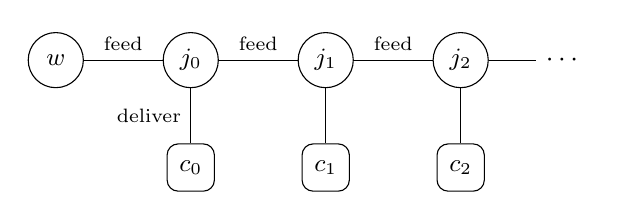
\begin{tikzpicture}[
  v/.style={circle, draw, inner sep=1.5pt, minimum size=7mm, font=\small},
  c/.style={rectangle, draw, rounded corners, inner sep=2pt, minimum size=6mm, font=\small}]
\node[v] (w) {$w$};
\node[v, right=1cm of w] (j0) {$j_0$};
\node[v, right=1cm of j0] (j1) {$j_1$};
\node[v, right=1cm of j1] (j2) {$j_2$};
\node[right=0.6cm of j2] (dots) {$\cdots$};
\node[c, below=0.7cm of j0] (c0) {$c_0$};
\node[c, below=0.7cm of j1] (c1) {$c_1$};
\node[c, below=0.7cm of j2] (c2) {$c_2$};
\draw (w) -- node[above, font=\scriptsize]{feed} (j0) -- node[above, font=\scriptsize]{feed} (j1)
  -- node[above, font=\scriptsize]{feed} (j2) -- (dots);
\draw (j0) -- node[left, font=\scriptsize]{deliver} (c0);
\draw (j1) -- (c1);
\draw (j2) -- (c2);
\end{tikzpicture}
\end{center}
Each junction has a \emph{feed} edge from its predecessor (the signal vertex itself for $j_0$)
and a \emph{deliver} edge to the vertex owning its consumer: the gate vertex of the slot, or
the acceptor.

\paragraph{The network.} The vertices are the signals, the junctions, and the acceptor; the
edges are the feed and deliver edges, two per junction (\lean{Frontier.Compiler.network}). The
constraints are:
\begin{itemize}
\item at the vertex of an input $x_i$, which reads $x_i$: its outgoing edge carries $x_i$;
\item at the vertex of a gate $g$: its outgoing edge carries $I(g)$ applied to the values on the
  deliver edges of its argument slots;
\item at a junction: both of its outgoing edges carry the value of its feed edge;
\item at the acceptor: its incoming edge carries a value in $\Acc$.
\end{itemize}

The design is uniform: a signal with a single consumer has a chain of length one, so there is
no special case for fan-out one, and the acceptor is just another consumer, so even a circuit
whose output is an input wire compiles without a special case.

\subsection{Exactness}

\begin{theorem}[Exactness]
\label{thm:exact}
The network accepts exactly the inputs on which the output lies in $\Acc$. For each accepted
input the satisfying assignment is unique: it is the run of the program.
\leanref{Frontier.Compiler.accepted_network}
\end{theorem}

\begin{proof}
If the output lies in $\Acc$, put on every edge the value of its signal in the run of the
program; every constraint holds (\lean{Frontier.Compiler.trace_satisfies}).
Conversely, let $\alpha$ satisfy the network. The junction constraints force every edge of a
signal to carry the value of the signal's first feed edge
(\lean{Frontier.Compiler.eq_head}). By induction along the program order, using that a gate
reads only inputs and earlier gates
(\lean{Cslib.Circuits.Program.lines_wires_eq_gate_lt}), the gate constraints force that value
to be the signal's value in the run (\lean{Frontier.Compiler.head_eq_trace}). The acceptor's
constraint then says that the output lies in $\Acc$.
\end{proof}

Uniqueness is not needed for the lower bound, which only uses one satisfying assignment per
input. It explains why the sweep is unambiguous: the local guesses of a sweep are forced
globally.

\subsection{Shape and size}

\begin{proposition}[Shape]
\label{prop:shape}
The network is connected and loopless. If the fan-in is at most $r \ge 2$, every vertex has
degree at most $r+1$; in particular, for fan-in two the graph is subcubic.
\leanref{Frontier.Compiler.maxDegreeLE}
\end{proposition}

\begin{proof}
A gate vertex has at most $r$ incoming deliver edges and one outgoing feed edge; a junction has
its feed, its deliver, and the feed of the next junction; an input vertex and the acceptor have
one edge each. Every vertex is joined to the acceptor: a junction along its chain to its
signal, and a signal through a consumer to that consumer's gate, which is joined to the
acceptor by induction on reachability (\lean{Frontier.Compiler.connected}). No edge joins a
vertex to itself (\lean{Frontier.Compiler.loopless}).
\end{proof}

\begin{proposition}[Counting]
\label{prop:counting}
Let the fan-in be at most $r$, and let $\rd$ be the set of reachable inputs, which are the
inputs read by the network. Then
\[
  \beta_1 + \card{\rd} \le (r-1)\,s + 1 \qquad\text{and}\qquad \card V \le n + (r+1)\,s + 2 .
\]
\leanref{Frontier.Compiler.cycleRank_add_ncard_read_le}
\end{proposition}

\begin{proof}
Let there be $C$ consumers, $W$ signals, $s'$ reachable gates and $m = \card{\rd}$ reachable
inputs. There are $2C$ edges and $W + C + 1$ vertices, so $\beta_1 = C - W$. Every slot belongs
to a reachable gate, so $C \le r s' + 1$, while $W = s' + m$. Hence
$\beta_1 + m \le (r-1)s' + 1 \le (r-1)s + 1$, and $\card V = W + C + 1 \le n + (r+1)s + 2$
(\lean{Frontier.Compiler.card_vertex_le}).
\end{proof}

For fan-in two the bound reads $\beta_1 \le s + 1 - m$. A formula on $m$ inputs has $m - 1$
binary gates and compiles to a tree: every gate beyond those of a formula adds one
independent cycle. Gates create local constraints; fan-out creates topology.

% ===========================================================================
\section{The lower bound}
\label{sec:lowerbound}

\subsection{The reduction theorem}

\begin{theorem}[Reduction]
\label{thm:reduction}
Let $c$ be a circuit of size $s$ and fan-in at most $r \ge 2$, over any basis on $U$, deciding a
$K$-rectangle-free set $S \subseteq U^n$ with $\card S \ge q K^2$. Then there is a connected,
loopless multigraph $G$ of maximum degree $r+1$ with
\[
  \card{V(G)} \le n + (r+1)s + 2 \qquad\text{and}\qquad
  \beta_1(G) \le (r-1)\,s - n + \log_q K + 1,
\]
every layout of which has width at least
\[
  \log_q \card S \;-\; 3 \log_q K \;-\; \log_q\bigl(\card{V(G)} + 1\bigr) \;-\; (r+2).
\]
\leanref{Frontier.exists_graph_of_decides}
\end{theorem}

\begin{proof}
Let $G$ be the constraint graph of $c$; its shape and size are given by
\cref{prop:shape,prop:counting}. The accepted set is $S$ (\cref{thm:exact}), which depends
only on the read inputs, so the support lemma gives $q^{n - \card{\rd}} < K$. Hence
$\card{\rd} > n - \log_q K$, and \cref{prop:counting} gives the bound on $\beta_1$
(\lean{Frontier.cycleRank_le}). For a layout of width $w$, \cref{thm:network-counting} with
$d = r+1$ and $m = 1$ gives
\[
  \card S \le (K-1)^2 \bigl(\card V q^{w + r + 2} + q^{n - \card{\rd}}\bigr)
          \le K^2 \bigl(\card V\, K q^{w+r+2} + K q^{w+r+2}\bigr)
          = K^3 (\card V + 1)\, q^{w + r + 2},
\]
using $q^{n - \card{\rd}} < K$ once more; take logarithms
(\lean{Frontier.logb_ncard_le}).
\end{proof}

For a dense set, $\log_q \card S \approx n$. So a circuit of size $s$ yields a graph of cycle rank
about $(r-1)s - n$ all of whose layouts have width about $n$: the circuit must be large unless
graphs of small cycle rank can be wide.

\subsection{Proof of the main theorem}

\begin{proof}[Proof of \cref{thm:main}]
Write $\lambda = \log q$ and $\sigma = (r-1)s$. Since a smaller $\varepsilon$ gives a stronger
statement, we may assume $A\varepsilon \le 1$. Choose the layout slack $\eta > 0$ with
$\eta(4 + 4/A) = A\varepsilon/2$, and let $C$ be the constant that $\LB_{r+1}(A)$ provides for
$\eta$. Set $\delta = A \varepsilon \lambda / 10$.

For large $n$ the hypotheses give $\card{S_n} \ge q K_n^2$, and
\[
  n \lambda - \log\card{S_n} \le \delta n, \qquad (A + \eta + 3)\log K_n \le \delta n, \qquad
  \log\bigl((4 + 3/A)n + 3\bigr) \le \delta n,
\]
together with $\bigl(A + 3\eta + C + r + 2\bigr) \lambda \le \delta n$. Suppose, for contradiction,
that a circuit of fan-in at most $r$ deciding $S_n$ has $\sigma \le (1 + 1/A - \varepsilon) n$.
Applying the layout bound to the graph of \cref{thm:reduction}, and using
$\card V \le n + (r+1)s + 2 \le n + 3\sigma + 2$ (as $r \ge 2$), we obtain after multiplying by
$\lambda$ (\lean{Frontier.logb_ncard_le_of_layout}):
\[
  \log\card{S_n} \le (A + \eta) \lambda(\sigma - n) + (A + \eta + 3)\log K_n
    + (A + 3\eta + C + r + 2) \lambda + \eta \lambda (n + 3\sigma) + \log(n + 3\sigma + 3).
\]
From $\sigma - n \le (1/A - \varepsilon) n$ we get
$(A + \eta) \lambda(\sigma - n) \le (1 - A\varepsilon + \eta/A)\,n\lambda$, and from
$\sigma \le (1 + 1/A)n$ we get $\eta \lambda(n + 3\sigma) \le \eta(4 + 3/A)\,n\lambda$; the choice of
$\eta$ makes the two $\eta$ terms sum to $(A\varepsilon/2)\,n\lambda$. The remaining terms are at most
$3\delta n$. So
\[
  n\lambda - \delta n \;\le\; \log\card{S_n} \;\le\; \Bigl(1 - \frac{A\varepsilon}{2}\Bigr) n\lambda + 3\delta n,
\]
that is, $(A\varepsilon/2)\,n\lambda \le 4\delta n = (2/5)\,A\varepsilon\, n\lambda$, which is false.
\end{proof}

The fixed-length inequality (\lean{Frontier.logb_ncard_le_of_layout}) keeps every lower-order
term explicit, and can be used for concrete parameters.

% ===========================================================================
\section{Layout bounds}
\label{sec:layouts}

This section proves the layout bound for subcubic graphs that \cref{thm:main} takes as input.
The coefficient is that of a random layout: score the edges of a cubic graph by correlated
Gaussians, and list the vertices by the median of their scores.

\begin{theorem}[Gaussian layouts]
\label{thm:layout}
Let $p = \frac{3}{2\pi}\arccos\frac{1 + 2\sqrt2}{4} \approx 0.14035$. Then $\LB_3(2p)$ holds,
and since $2p \le 9/32$, so does $\LB_3(1/3)$.
\leanref{Frontier.layoutBound_gaussian}
\end{theorem}

The proof has three parts. \Cref{sec:cubic} reduces subcubic multigraphs to simple cubic
graphs, at the cost of the factor two. \Cref{sec:median} reduces laying out a cubic graph to
scoring its edges. \Cref{sec:gaussian} chooses the scores.

\subsection{Reduction to cubic graphs}
\label{sec:cubic}

Call a simple cubic graph on $h$ vertices \emph{$c$-layable} if for every $\xi > 0$ and all
large $h$ it has a layout whose frontiers have at most $(c + \xi) h + 2$ edges
(\lean{Frontier.CubicLayoutBound}).

\begin{proposition}[Compression]
\label{prop:compression}
If large cubic graphs are $c$-layable, then $\LB_3(2c)$ holds.
\leanref{Frontier.LayoutBound.of_cubic}
\end{proposition}

\begin{proof}[Proof sketch]
Let $G$ be connected, loopless, and subcubic. Partition its vertices into \emph{blocks}, each
an ordered list, starting from singletons, and repeatedly merge two adjacent blocks when one
has at most two edges leaving it or they are joined by parallel edges, listing the larger block
first. Three invariants are kept: every block has at most three edges leaving it; every proper
prefix of a block of size $b$ has at most $3\lceil\log_2 b\rceil$ edges leaving it, because a
prefix of a merged block is a prefix of the larger part or the larger part followed by a prefix
of the smaller part, which has at most half the size; and the number of blocks plus the number
of edges inside blocks is at least $\card V$, since every merge absorbs an edge. When no merge
applies and at least two blocks remain, the quotient graph $H$ on the blocks is simple and
cubic, and the last invariant gives $h + 2\card V \le 2\card E$, that is,
$h \le 2(\beta_1(G) - 1)$. Lay out $G$ block by block in the order of a layout of $H$, each
block in its recorded order. A frontier is then a frontier of $H$ together with the boundary of
one partial block, so it has at most $(c + \xi)\,2\beta_1(G) + 3\log_2\card V + O(1)$ edges, and
the logarithm is absorbed into $\eta\card V + C$.
\end{proof}

\subsection{Median layouts}
\label{sec:median}

Give each edge $e$ of a cubic graph a real \emph{score} $s(e)$. Each vertex has three edges and
hence a \emph{median} score $m(v)$: at least two of its edges score at most $m(v)$, and at
least two score at least $m(v)$. A vertex \emph{straddles} a threshold $\theta$ if one of its
edges scores below $\theta$ and another at least $\theta$. The \emph{median layout} lists the
vertices by median score, breaking ties arbitrarily.

\begin{lemma}[Median layouts]
\label{lem:median}
Fix a grid $a, a + \delta, \dots, a + M\delta$, and let $B$ be at least three times the number
of edges scoring below $a$, at least three times the number scoring at least $a + M\delta$,
and, for every $i < M$, at least
\[
  \#\{v \text{ straddling } a + i\delta\} \;+\;
  3\,\#\{e : a + i\delta \le s(e) < a + (i+1)\delta\}.
\]
Then every frontier of the median layout has at most $B$ edges.
\leanref{Frontier.exists_key_of_edgeScore}
\end{lemma}

\begin{proof}
Let $P$ be an initial segment of the layout and choose $m$ with $m(u) \le m$ for $u \in P$ and
$m(v) \ge m$ for $v \notin P$. An edge $e = uv$ leaving $P$, with $u \in P$, is charged as
follows. If $s(e) < \theta \le m$ for a threshold $\theta$, charge $e$ to $v$: then
$s(e) < m(v)$, and at most one edge at $v$ scores below its median, so $v$ is charged at most
once. If $s(e) \ge \theta' > m$, charge $e$ to $u$: then $s(e) > m(u)$, and at most one edge at
$u$ scores above its median.

If $a + i\delta \le m < a + (i+1)\delta$, take $\theta = a + i\delta$ and
$\theta' = a + (i+1)\delta$. A vertex $v \notin P$ charged by an edge below $\theta$ has two
edges scoring at least $m(v) \ge \theta$, so it straddles $\theta$. A vertex $u \in P$ charged by
an edge at least $\theta'$ has two edges scoring at most $m(u) < \theta'$: if one scores below
$\theta$, then $u$ straddles $\theta$; otherwise $u$ is an endpoint of an edge scoring in the
window $[\theta, \theta')$. The remaining edges leaving $P$ score in the window. Since a window
edge has two endpoints, at most $\#\{\text{straddlers}\} + 3\,\#\{\text{window edges}\}$ edges
leave $P$. If $m < a$, every edge leaving $P$ scores below $a$ or is charged to a vertex of $P$
with two edges below $a$, so at most three times the edges below $a$ leave $P$; the case
$m \ge a + M\delta$ is symmetric.
\end{proof}

\Cref{lem:median} replaces the path decompositions through which such scores are usually
turned into layouts: a frontier of the median layout is bounded directly by straddling counts.

\subsection{Gaussian edge scores}
\label{sec:gaussian}

Let $H$ be a simple cubic graph with vertex set $V$. For a decay rate $0 \le q < 1/\sqrt2$ and a
radius $R$, the \emph{kernel row} of a vertex $v$ is the vector in $\R^V$ with entries
$q^{\mathrm{dist}(v, z)}$ for $\mathrm{dist}(v,z) \le R$ and $0$ otherwise; let $x_v$ be its
normalization (\lean{Frontier.Gaussian.unitKernel}). For an edge $uv$ let $y_{uv}$ be the unit
vector in the direction of $x_u + x_v$. Draw a standard Gaussian vector $\omega \in \R^V$ and
score each edge by $s(e) = \langle y_e, \omega\rangle$.

\begin{lemma}[Kernel correlation]
\label{lem:kernel}
In a graph of maximum degree three, adjacent unit kernel rows satisfy
$\langle x_u, x_v\rangle \ge 2q/(1+q^2) - 3(2q^2)^R$.
\leanref{Frontier.Gaussian.sum_unitKernel_mul_ge}
\end{lemma}

\begin{proof}[Proof sketch]
For adjacent $u, v$ the distances $d_u = \mathrm{dist}(u,z)$ and $d_v = \mathrm{dist}(v,z)$ differ
by at most one, so $q^{d_u} q^{d_v} \ge \frac{2q}{1+q^2}\cdot\frac{q^{2d_u} + q^{2d_v}}{2}$,
which needs no girth assumption. Summing over $z$ gives the bound up to the vertices at the
truncation radius: the sphere of radius $R$ has at most $3 \cdot 2^{R}$ vertices in maximum
degree three, and they contribute at most $3(2q^2)^R$.
\end{proof}

\begin{lemma}[Sheppard's bound at every threshold]
\label{lem:sheppard}
For unit vectors $\alpha, \beta$ with $\langle\alpha,\beta\rangle = \rho > -1$ and any threshold
$\theta$, the probability that $\theta$ separates $\langle \alpha,\omega\rangle$ and
$\langle\beta,\omega\rangle$ is at most $\arccos(\rho)/\pi$.
\leanref{Frontier.Gaussian.gaussPi_between_le_arccos}
\end{lemma}

\begin{proof}
The forms $S = \langle\alpha + \beta, \omega\rangle$ and $D = \langle\beta - \alpha,\omega\rangle$ are
uncorrelated jointly Gaussian, hence independent, and a separation forces
$\lvert S - 2\theta\rvert \le \lvert D\rvert$. Conditionally on $D$, a centered Gaussian gives a
symmetric interval at least the mass of any translate (Anderson's inequality on the line), so
the probability is at most $\Pr[\lvert S\rvert \le \lvert D\rvert]$. By the planar angle law this
is $\frac{2}{\pi}\arctan\sqrt{(1-\rho)/(1+\rho)} = \arccos(\rho)/\pi$.
\end{proof}

\begin{proposition}[One vertex]
\label{prop:straddle}
If adjacent kernel rows have correlation at least $\rho_0 \ge 17/32$, a vertex straddles any
fixed threshold with probability at most $\frac{3}{2\pi}\arccos\frac{1 + 3\rho_0}{4}$.
\leanref{Frontier.Gaussian.measureReal_straddleEvent_le}
\end{proposition}

\begin{proof}
A straddling vertex has at least four separated ordered pairs among its three edges, so the
probability is at most a quarter of the sum, over the six ordered pairs, of the separation
probabilities, each at most $\arccos(\rho')/\pi$ by \cref{lem:sheppard}. Each edge vector at
$v$ has correlation $\sqrt{(1+\rho)/2} \ge \kappa = \sqrt{(1+\rho_0)/2}$ with $x_v$. Since
$\lVert\sum_e y_e\rVert \ge \langle \sum_e y_e, x_v\rangle \ge 3\kappa$, the pairwise correlations
average at least $(3\kappa^2 - 1)/2 = (1 + 3\rho_0)/4$, and as $\arccos$ is concave and decreasing
on $[0,1]$, the six angles sum to at most $6\arccos\frac{1+3\rho_0}{4}$
(\lean{Frontier.Gaussian.sum_arccos_star_le}).
\end{proof}

\begin{proof}[Proof of \cref{thm:layout}]
Fix thresholds $-T + i\delta$ for $i \le M$, with $\delta = 2T/M$. The number of straddling
vertices at a threshold, the number of edges scoring in a window, and the number of edges in
each tail are sums of events, each depending only on the coordinates of $\omega$ in a ball of
radius $R + 1$. Each ball meets boundedly many others, so each count has variance $O(h)$ and,
by Chebyshev's inequality, lies within $\varepsilon h$ of its mean except with probability
$O(1/(\varepsilon^2 h))$ (\lean{Frontier.Gaussian.pi_deviation_le}). The means are at most
$\frac{3}{2\pi}\arccos\frac{1+3\rho_0}{4}\,h$ for straddlers (\cref{prop:straddle}),
$\frac32 h \cdot \delta/\sqrt{2\pi}$ for window edges, and $\frac32 h/T^2$ for each tail. For
large $h$ a union bound over the $2M + 2$ counts leaves some $\omega$ for which all of them are
near their means, and \cref{lem:median} bounds every frontier of its median layout by
\[
  h\cdot\max\Bigl(\tfrac{9}{2T^2} + 3\varepsilon,\
  \tfrac{3}{2\pi}\arccos\tfrac{1+3\rho_0}{4} + \tfrac{9\delta}{2\sqrt{2\pi}} + 4\varepsilon\Bigr)
\]
(\lean{Frontier.Gaussian.exists_good_sample}). Let $q \uparrow 1/\sqrt2$ and $R \to \infty$:
the correlation of \cref{lem:kernel} tends to $2\sqrt2/3$, the neighbour correlation of
Gaussian waves on the $3$-regular tree~\cite{CGHV2015,Lyons2017}, and
$(1 + 3\cdot 2\sqrt2/3)/4 = (1 + 2\sqrt2)/4$. Choosing $T$, $M$ and $\varepsilon$ to make the
other terms small shows that large cubic graphs are $p$-layable
(\lean{Frontier.Gaussian.cubicLayoutBound_gaussian}), and \cref{prop:compression} gives
$\LB_3(2p)$. The bound $2p \le 9/32$ follows from $\cos(3\pi/32) \le (1 + 2\sqrt2)/4$.
\end{proof}

\begin{corollary}[The unconditional bounds]
\label{cor:unconditional}
Under the hypotheses of \cref{thm:main} on $S_n$, every circuit of fan-in at most two deciding
$S_n$, over any basis, has more than $(L - \varepsilon)\,n$ gates for all large $n$, where
$L = 1 + \pi \big/ \bigl(3\arccos\frac{1+2\sqrt2}{4}\bigr) \approx 4.5625$; in particular more
than $(4 - \varepsilon)\,n$ gates.
\leanref{Frontier.lowerBound_gaussian}
\end{corollary}

The coefficient $1/3$ was known earlier, from the cubic bisection bound of Monien and
Preis~\cite{MonienPreis2006} and the resulting pathwidth bound of Fomin and
H{\o}ie~\cite{FominHoie2006}; here it is a consequence of \cref{thm:layout}.

\subsection{Limits of edge layouts}

Random cubic graphs on $h$ vertices have bisection width at least $0.103295\,h$ with high
probability~\cite{LichevMitsche2020}, and the cutwidth of a graph is at least its bisection
width, since the middle frontier of any layout is a bisection. A cubic graph on $h$ vertices
has cycle rank $h/2 + 1$, so $\LB_3(A)$ is false for $A < 0.2066$: with the layout bound as its
only graph-theoretic input, the method cannot give a coefficient above
$1 + 1/0.2066 \approx 5.84$ for fan-in two. Larger coefficients would
need a finer measure of frontiers than their number of edges, or a different compiler.

\subsection{Larger fan-in}

For fan-in $r \ge 3$ one needs $\LB_{r+1}(A)$ for graphs of maximum degree $r+1$, and any such
bound gives $(r-1)s > (1 + 1/A - \varepsilon)\,n$. Since every circuit computing a function of
$n$ essential variables has $(r-1)s \ge n - 1$, the method improves the trivial bound by the
factor $1 + 1/A$. We do not know the best coefficients for $d \ge 4$; a compression as in
\cref{sec:cubic} should again reduce the question to graphs of minimum degree three.

% ===========================================================================
\section{Design notes on the formalization}
\label{sec:design}

The formal statements are meant to be read. We record the choices behind them.

\paragraph{Faithful, minimal statements.}
The main theorem quantifies over every signature, interpretation, acceptance set, and circuit
at once, and its hypotheses are exactly those of \cref{thm:main}: rectangle-freeness,
$\log K_n = o(n)$, density, and $\LB_{r+1}(A)$. The density hypothesis is stated as
$n \log q - \log\card{S_n} = o(n)$ and the threshold hypothesis as $\log K_n = o(n)$, with
Mathlib's little-$o$.

\paragraph{Sets and cardinalities.}
Sets of inputs, rectangles, cuts, and edge neighbourhoods are \lean{Set}s, and sizes are
\lean{Set.ncard} and \lean{Nat.card}. No statement mentions decidability, and finiteness enters
only as \lean{Finite} instances on coordinates, alphabet, vertices, and edges. Proofs pass to
\lean{Finset} when they need its counting lemmas; the two needed fiber-counting estimates are
stated for \lean{Set.ncard} in \lean{Frontier/ForMathlib/SetCard.lean}.

\paragraph{The sweep lemma is abstract.}
\Cref{lem:counting} is stated for an abstract sweep (\lean{Frontier.Sweep}) and proved without
reference to graphs. Messages are arbitrary functions into an arbitrary type; for networks they
are frontier values, encoded as functions $E \to \mathrm{Option}\ U$ that are \texttt{none}
off the frontier. The revealed sets need not be nested. This makes the lemma reusable: any
object that produces a sweep, such as a branching program or a different compiler, inherits the
counting.

\paragraph{Inputs and sites.}
Each input is read by at most one vertex, so the site map is
$\iota \to \mathrm{Option}\ V$. Inputs that no vertex reads are revealed in one extra step at
the end of the sweep. This keeps the network definition honest, since an unread input is
simply not read, and places the cost of unread inputs exactly where the support lemma pays for
it.

\paragraph{Locality as an axiom of the structure.}
A constraint is a predicate on a whole input and a whole edge assignment, together with a
field asserting that it depends only on the incident edges and the inputs read at the vertex.
Encoding constraints as predicates on dependent function types $U^{E(v)}$ would make locality
definitional, but at the cost of transport along the incidence relation in every proof.

\paragraph{Junction chains.}
A signal of fan-out $f \ge 2$ can be routed through only $f - 1$ copy vertices, but at the cost
of special cases for fan-out one and for the last pair of consumers. One junction per consumer,
with the junctions of a signal numbered by an equivalence between consumers and pairs (signal,
position), removes every special case at the cost of one extra vertex and one extra edge per
signal, which changes neither the cycle rank nor the theorem.

\paragraph{Witnesses, not uniqueness.}
The sweep of a network chooses a satisfying assignment for each accepted input with Hilbert's
choice operator. Uniqueness of the satisfying assignment holds for compiled circuits
(\cref{thm:exact}) but is never used, so the network results apply verbatim to
nondeterministic constraint systems.

\paragraph{The layout hypothesis.}
$\LB_d(A)$ quantifies over graphs whose vertex and edge types live in \lean{Type}, with
\lean{Finite} instances, and asks for a layout as an equivalence $V \simeq \mathrm{Fin}\,\card V$.
The error term $\eta\card V + C$ is the weakest form that suffices, so the hypothesis is as weak
as possible; in the proof of \cref{thm:layout} it absorbs the logarithmic boundaries of the
compression blocks.

\paragraph{Median layouts instead of path decompositions.}
Edge scores are usually turned into vertex layouts through path decompositions: list the edges
by score, keep each vertex in the bags between its first and last edge, and order the vertices
by the median of their bags. \Cref{lem:median} goes directly from scores to frontiers, which
removes path decompositions from the development.

\paragraph{Upstreaming.}
Three facts about CSLib programs (\lean{Frontier/ForCslib/Program.lean}): a gate reads only
earlier gates, a fan-in bound bounds every line's arity, and a gate's value is its operation
applied to its arguments' values. The constraint network and the compiler would fit naturally in
CSLib next to its circuit model.

% ===========================================================================
\section{Extensions}
\label{sec:extensions}

\paragraph{Arithmetic circuits and rank.}
Over an infinite field $\mathbb F$ the counting of \cref{lem:counting} is meaningless, but the
compiler and the separator lemma are unchanged. For a circuit computing a linear map
$x \mapsto Mx$, differentiating at a point attaches to each wire a row vector, and the
separator lemma becomes a rank inequality: the influence of the inputs on one side of a cut on
the outputs on the other side factors through the span of the frontier rows. For totally
regular matrices, such as Cauchy matrices, the same argument gives the coefficient $1 + 1/A$
for arithmetic circuits of fan-in two computing all outputs, over every field. The general
shape is
\begin{align*}
  \text{bounded-arity circuit} \;&\to\; \text{bounded-degree constraint graph} \\
  &\to\; \text{small frontier} \;\to\; \text{semantic capacity of that frontier},
\end{align*}
where counting, rank, and other capacities occupy the last step.

\paragraph{Nondeterministic circuits.}
Witness inputs can be read anywhere in the network and existentially quantified; since the
sweep never uses uniqueness, the same argument gives the same bound counting only the ordinary
inputs.

\paragraph{Better layouts.}
Any improvement of $\LB_3(A)$ below $A = 0.2807$ improves \cref{cor:fanin-two} immediately.
Numerical experiments suggest that nonlinear smoothing of Gaussian edge scores helps, but no
proof is known.

% ===========================================================================
\appendix
\section{Index of formal statements}
\label{app:index}

All declarations are in the namespace \lean{Frontier}, in the file of the same name under
\lean{Frontier/}, except for the upstreaming candidates in \lean{Frontier/ForMathlib} and
\lean{Frontier/ForCslib}.

\begin{center}
\small
\begin{tabular}{ll}
\toprule
Paper & Lean declaration \\
\midrule
\multicolumn{2}{l}{\emph{Rectangles} (\lean{Rectangle.lean})} \\
Def.~\ref{def:rectangle} & \lean{rectangle} \\
Def.~\ref{def:rectangle-free} & \lean{RectangleFree} \\
Lem.~\ref{lem:ignored} & \lean{RectangleFree.ncard_le_of_dependsOn} \\
Lem.~\ref{lem:support} & \lean{RectangleFree.pow_ncard_compl_lt} \\
\midrule
\multicolumn{2}{l}{\emph{Sweeps} (\lean{Sweep.lean})} \\
Def.~\ref{def:sweep} & \lean{Sweep}, \lean{Sweep.transition} \\
Lem.~\ref{lem:counting} & \lean{Sweep.ncard_le} \\
\midrule
\multicolumn{2}{l}{\emph{Graphs and networks} (\lean{Multigraph.lean}, \lean{Network.lean})} \\
Hyp.~\ref{hyp:layout} & \lean{LayoutBound} \\
Def.~\ref{def:network} & \lean{Network}, \lean{Network.accepted} \\
Lem.~\ref{lem:separator} & \lean{Network.Satisfies.splice} \\
Prop.~\ref{prop:network-sweep} & \lean{Network.sweep} \\
Thm.~\ref{thm:network-counting} & \lean{Network.ncard_accepted_le} \\
\midrule
\multicolumn{2}{l}{\emph{Compiler} (\lean{Compiler.lean})} \\
Thm.~\ref{thm:exact} & \lean{Compiler.accepted_network} \\
Prop.~\ref{prop:shape} & \lean{Compiler.maxDegreeLE} \\
 & \lean{Compiler.connected}, \lean{Compiler.loopless} \\
Prop.~\ref{prop:counting} & \lean{Compiler.cycleRank_add_ncard_read_le} \\
 & \lean{Compiler.card_vertex_le} \\
\midrule
\multicolumn{2}{l}{\emph{Lower bound} (\lean{Reduction.lean}, \lean{LowerBound.lean})} \\
Thm.~\ref{thm:reduction} & \lean{exists_graph_of_decides} \\
Thm.~\ref{thm:main} & \lean{lowerBound} \\
Cor.~\ref{cor:fanin-two} & \lean{lowerBound_fanInTwo} \\
\midrule
\multicolumn{2}{l}{\emph{Layouts} (\lean{Layouts/*.lean}, \lean{Layouts.lean}, \lean{Main.lean})} \\
Thm.~\ref{thm:layout} & \lean{layoutBound_gaussian}, \lean{layoutBound_one_third} \\
Prop.~\ref{prop:compression} & \lean{LayoutBound.of_cubic} \\
Lem.~\ref{lem:median} & \lean{exists_key_of_edgeScore} \\
Lem.~\ref{lem:kernel} & \lean{Gaussian.sum_unitKernel_mul_ge} \\
Lem.~\ref{lem:sheppard} & \lean{Gaussian.gaussPi_between_le_arccos} \\
Prop.~\ref{prop:straddle} & \lean{Gaussian.measureReal_straddleEvent_le} \\
Cor.~\ref{cor:unconditional} & \lean{lowerBound_gaussian}, \lean{lowerBound_four} \\
\bottomrule
\end{tabular}
\end{center}

\bibliographystyle{alpha}
\bibliography{references}

\end{document}
